\documentclass{article}
\usepackage{graphicx} % Required for inserting images
\usepackage{subfig}
% \usepackage{subcaption}
\usepackage{amsmath}
\usepackage{algorithmicx}
\usepackage{algpseudocode}
\usepackage{amssymb}
\usepackage[margin=1in]{geometry}
\usepackage{url}
\usepackage{changepage}



\title{ECSE 4850 - Programming Assignment 3}
\author{Philip Paterson}
\date{March 2024}

% Set learning rate variable
\newcommand{\learningrate}{0.006}
\newcommand{\testaccuracy}{72.8}
\newcommand{\testerror}{27.2}
\newcommand{\batchsize}{64}
\newcommand{\epochs}{100}
\newcommand{\momentum}{0.9}

\begin{document}

\maketitle

\section{Introduction - Problem Statement}
% A brief introduction to the problem you are going to solve. Summarize the task in your own words. Do not copy the sentences from the instruction.
In Programming Assignment 3, we program a convolutional neural network (CNN) with three convolutional layers, two max-pooling layers, and two fully-connected layers, to perform multi-class classification to classify images into 10 classes in the CIFAR-10 dataset.

The 10 classes in the CIFAR-10 dataset are as follows: "truck," "ship," "horse," "frog," "dog," "deer," "cat," "bird," "automobile," and "airplane." In the dataset there are 60,000 images, with 50,000 being part of the training set and 10,000 being part of the testing set. Each image is a 3-channel colored 32x32x3 image.

In this report, I will describe the structure of the model used, how the experiment was set up, the results of my experiments, analysis on my results, and make concluding remarks.

\section{Model Description}
% Clearly describe your model including the structure.  You should discuss model components such as input and layer sizes, filter sizes, and activation functions.  You should include an illustration of the architecture.

\subsection{Data Augmentation}
I first transformed my data by performing horizontal and vertical flips on the images with the probability of being flipped being $p=0.5$.

\subsection{Convolutional Neural Network Architecture}
% input shape: torch.Size([5000, 3, 32, 32])
% After conv1 shape: torch.Size([5000, 16, 28, 28])
% After pooling 1 shape: torch.Size([5000, 16, 14, 14])
% After conv2 shape: torch.Size([5000, 32, 10, 10])
% After pooling 2 shape: torch.Size([5000, 32, 5, 5])
% After conv3 shape: torch.Size([5000, 64, 3, 3])
% before fc1 x shape: torch.Size([5000, 576])
% After connected layer 1 torch.Size([5000, 500])
% Output: torch.Size([5000, 10])

My model is a Convolutional Neural network with the following layers: three convolutional layers, two max-pooling layers, and two fully-connected layers. The ReLU activation function is used between the convolution layers and max-pool layers, along as being used between the last convolutional layer and first fully-connected layer and between the first and second fully-connected layers. In addition, to avoid overfitting, batch normalization is used between the convolution and activation layers, as well as dropout being utilized between the first and second fully connected layers.

Please note that when I describe my dimensions, I will be using the  convention of (height x width x depth) for a three-dimensional tensor. Thus, a 32x32x3 image has a depth of 3, or 3 channels, and a height and width of 32.

\subsubsection{Mathematical Description}
\label{subsubsec:cnn_math}

We first will cover the convolutional layer. Let $\textbf{X}^{M \times N \times D}$ be the input image with D channels. Thus, for the CIFAR-10 dataset, $M = N = 32$ and $D=3$. Additionally, define $\textbf{W}^{c ~ K \times K \times D}$ as the filter and $\textbf{W}_0^c$ as the bias. Also, let the convolutional layer be $\textbf{C}^{N^c_r \times N^c_c}$ with stride $s$ (assuming zero-padding), where $N^c_r = \frac{M-k}{s}+1$ and $N^c_c = \frac{N-k}{s}+1$ are the height and width respectively. Thus, $\textbf{C}$ can be calculated as follows:\newline
\noindent For r = 1 to $N^c_r$ \newline
\noindent For c = 1 to $N^c_c$ \newline
\begin{equation*}
    \textbf{C}[r][c] = \sum_{l=1}^{D} \sum_{i=1}^{K} \sum_{j=1}^{K} \textbf{X}[(r-1) \times s + i][(c-1) \times s + j][l]\textbf{W}^{c}[i][j][l] + \textbf{W}_{0}^{c}
\end{equation*}

Next, to cover the convolution to activation layer $\textbf{A}^{N^a_r \times N^a_c}$, where $N^a_r=N^c_r$ and $N^a_c=N^c_c$. \newline
\noindent For r = 1 to $N^a_r$ \newline
\noindent For c = 1 to $N^a_c$ \newline
\begin{equation*}
    \textbf{A}[r][c] = \text{ReLU}(\textbf{C}[r][c])
\end{equation*}

Afterwards, from the activation layer to the pooling layer. If we define the pooling neighborhood size to be $d \times d$ and the pooling layer as $\textbf{P}^{N^p_r \times N^p_c}$, where $N^p_r = \frac{N^a_r-d}{s}+1$ and $N^p_c = \frac{N^a_c-d}{s}+1$ and $s$ is the pooling stride, the max-pooling layer can be calcualted as follows:\newline
\noindent For r = 1 to $N^c_r$ \newline
\noindent For c = 1 to $N^c_c$ \newline
\begin{equation*}
    \textbf{P}[r][c] = \max_{1 \leq i \leq d, 1 \leq j \leq d} \textbf{A}[(r - 1) \times s + i][(c - 1) \times s + j]
\end{equation*}

From the pooling layer to the fully connected layer, we first need to vectorize $\textbf{P}$ to $\vec{P}$. This can be done as follows:
\begin{algorithmic}
    \For{$r = 1$ to $N_r^p$}
        \For{$c = 1$ to $N_c^p$}
            \State $\vec{P}[(r - 1)N_c^p + c] = P[r][c]$
        \EndFor
    \EndFor
\end{algorithmic}

Afterwrds, the fully connected layer $\textbf{F}\in \mathbb{R}^{N^F \times 1}$ can be found as follows:
\begin{equation*}
    \textbf{F} = \phi((\textbf{W}^F)^T\vec{P} + \textbf{W}_0^F),
\end{equation*}
where $\phi$ is the activation function, $\textbf{W}^F$ are the weights, and $\textbf{W}_0^F$ is the bias.

After propagating forward throughout all the layers, the output layer can be calculated as follows:
\begin{equation*}
    \hat{y} = g\left((\textbf{W}^{o})^{T}\textbf{F} + \textbf{W}_{0}^{o}\right)
\end{equation*}
where $g$ is the output function (which is the softmax function in this model), $\textbf{W}^{o}$ are the output layer weights and $\textbf{W}_{0}^{o}$ is the bias.

\subsubsection{CNN Architecture Overview}
The following layers and dimensions of layers in Table \ref{table:cnn_layers} can be calculated using the equations in the previous section, section \ref{subsubsec:cnn_math}.

\begin{table}[h!]
    \centering
    \begin{tabular}{|l|l|}
    \hline
    \textbf{Layer} & \textbf{Dimensions $(H \times W \times D)$} \\
    \hline
    Input & $32 \times 32 \times 3$ \\
    Batch Normalization (2D) & - \\
    Convolutional Layer 1 (16 5$\times$5 filters) & $28 \times 28 \times 16$ \\
    Batch Normalization (2D) & - \\
    ReLU Activation & - \\
    After Max Pooling 1 (Pooling Area: 2$\times$2; Stride: 2) & $14 \times 14 \times 16$ \\
    Convolutional Layer 2 (32 5$\times$5 filters)& $10 \times 10 \times 32$ \\
    Batch Normalization (2D) & - \\
    ReLU Activation & - \\
    After Max Pooling 2 (Pooling Area: 2$\times$2; Stride: 2)& $5 \times 5 \times 32$ \\
    Convolutional Layer 3 (64 3$\times$3 filters)& $3 \times 3 \times 64$ \\
    Batch Normalization (2D) & - \\
    ReLU Activation & - \\
    Flatten & $576$ \\
    Fully Connected Layer 1 & $500$ \\
    ReLU Activation & - \\
    Dropout (p = 0.1) & - \\
    Fully Connected Layer 2 & $10$ \\
    Sigmoid Activation & - \\
    Output & - \\
    \hline
    \end{tabular}
    \caption{Convolutional Neural Network Layers and Dimensions}
    \label{table:cnn_layers}
\end{table}

\subsubsection{CNN Model Visualization}
The CNN model visualization can be seen in Figure \ref{fig:model_vis}.
\begin{adjustwidth}{-0.25in}{-0.25in}
    \begin{figure}[]
        \centering
        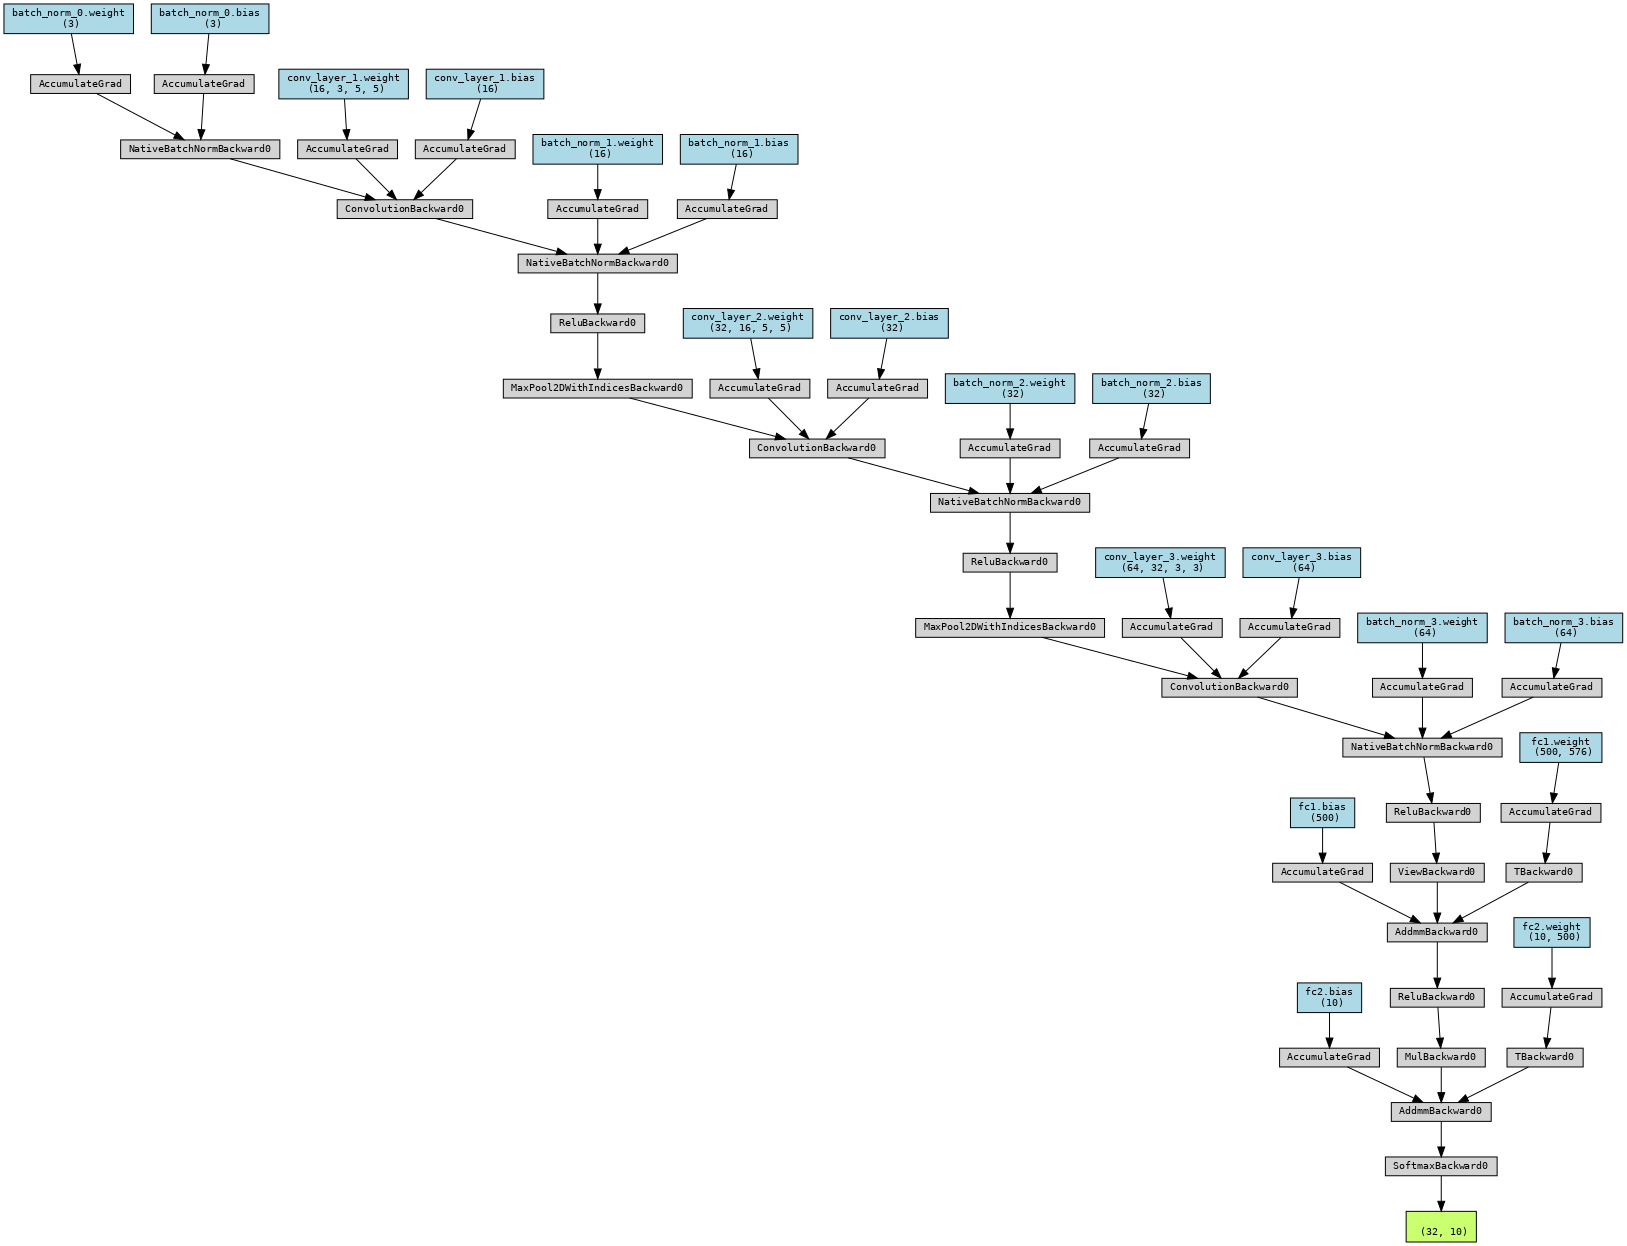
\includegraphics[width=7.25in]{plots_final/cnn_torchviz.png}
        \caption{torchviz visualization}
        \label{fig:model_vis}
    \end{figure}
\end{adjustwidth}

\section{Experimental Setup}
% Describe how you set up your experiments. You can talk about how the training and testing split is performed. Also, you can report your batch size, how you initialize the weight matrix, how you change the learning rate or any other hyper-parameter you used.
Here I will describe the setup of the experiments.
\subsection{The CIFAR-10 Dataset Split}
The 10 classes in the CIFAR-10 dataset are as follows: "truck," "ship," "horse," "frog," "dog," "deer," "cat," "bird," "automobile," and "airplane."

In the dataset there are 60,000 images, with 50,000 being part of the training set and 10,000 being part of the testing set. Each image is a 3-channel colored 32x32x3 image.

\subsection{Hyper parameters}
\begin{itemize}
    \item Batch size: \batchsize
    \item Epochs: \epochs
    \item Optimizer: Stochastic Gradient Descent (\verb|torch.optim.SGD|) \begin{itemize}
        \item Learning Rate = \learningrate
        \item Momentum = \momentum
        \end{itemize}
\end{itemize}

\subsection{Weight Initialization}
The weight initialization was performed using the default PyTorch weight initialization when an instance of the model is created. For example, for linear layers, PyTorch initializes weights using following formula (from \url{https://github.com/pytorch/pytorch/blob/main/torch/nn/modules/linear.py}):
\begin{equation*}
    \mathcal{U}(-\sqrt{k}, \sqrt{k})
\end{equation*}
where
\begin{equation*}
    k = \frac{1}{\text{in feature number}}
\end{equation*}

And initializes the convolutional layer weights using a uniform distribution between a positive and negative standard deviation, derived from the input channels (source: \url{https://github.com/pytorch/pytorch/blob/08891b0a4e08e2c642deac2042a02238a4d34c67/torch/nn/modules/conv.py#L40-L47}).

\section{Experimental Results}
% Plot the figure of training losses versus epochs. Plot the figure of training and testing accuracy versus epochs.  Report confusion matrix of classification.  Report the average classification error on the test dataset.

Average Classification Error on the Test Dataset: $\testerror \%$ \\
Average Classification Accuracy on the Test Dataset: $\testaccuracy \%$

The following figures describe my experimental results:
\begin{itemize}
    \item Average loss versus epochs: Figure \ref{fig:loss_vs_epochs}
    \item Average accuracy vs epochs: Figure \ref{fig:accuracy_vs_epochs}
    \item Confusion Matrix for the 10 classes: Figure \ref{fig:conf-mat}
\end{itemize}


\begin{figure}[]
    \centering
    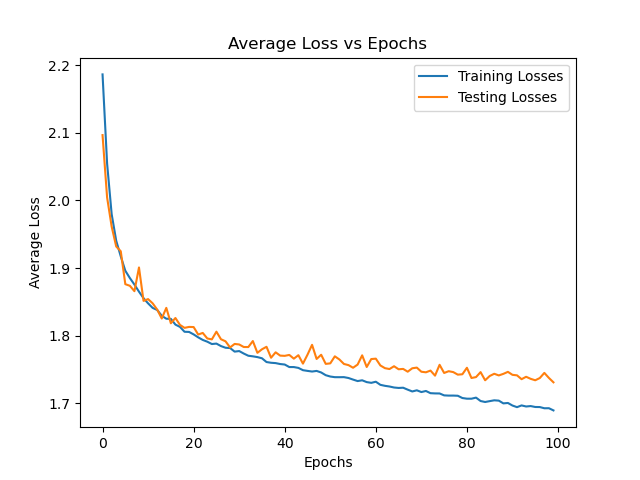
\includegraphics[width=5in]{plots_final/Average_Loss_vs_Epochs_plot.png}
    \caption{Average Loss vs Epochs}
    \label{fig:loss_vs_epochs}
\end{figure}

\begin{figure}[]
    \centering
    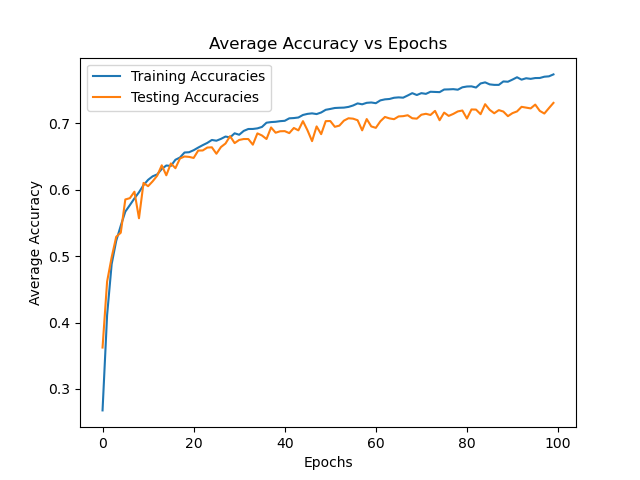
\includegraphics[width=5in]{plots_final/Average_Accuracy_vs_Epochs_plot.png}
    \caption{Average Accuracy vs Epochs}
    \label{fig:accuracy_vs_epochs}
\end{figure}

\begin{figure}[]
    \centering
    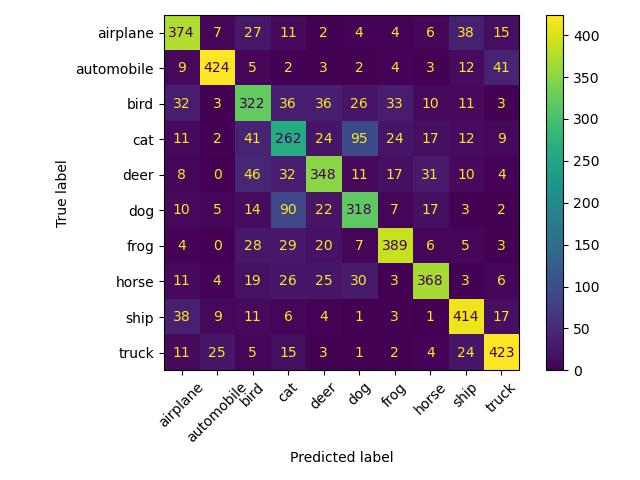
\includegraphics[width=5in]{plots_final/class_confusion_matrix.jpg}
    \caption{Confusion Matrix for 10 classes in CIFAR-10 Dataset}
    \label{fig:conf-mat}
\end{figure}

\section{Analysis}
% Visualization of the filters in your first convolutional layer. Please refer to the example in Figure 2. Based on your setup and results, analyze your results. High-quality analysis will get full marks.  Be creative here!

% label 0: airplane
% label 1: automobile
% label 2: bird 
% label 3: cat
% label 4: deer
% Label 5: dog
% Label 6: frog
% label 7: horse
% label 8: ship
% label 9: truck

\begin{figure}[]
    \centering
    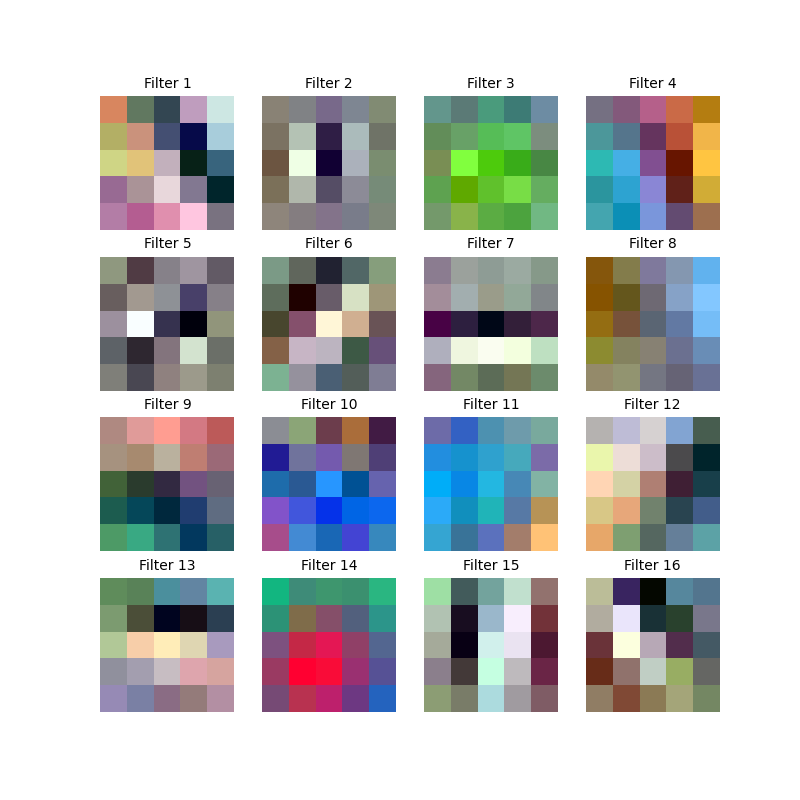
\includegraphics[width=5in]{plots_final/filters.png}
    \caption{16 Filters for the first Convolutional Layer}
    \label{fig:filters}
\end{figure}

The visualization of my filters can be seen in Figure \ref{fig:filters}.

Based on my setup and results, I was able to achieve an average test accuracy of $\testaccuracy\%$, which was about $4-5\%$ below my train accuracy.

In order to achieve this accuracy, the biggest factor that helped was batch regularization, as it allowed for faster convergence without as much overfitting. I believe this was because there was much variation in the input dataset, which regularization helps with by not being as affected by outliers.

I also further reduced overfitting using dropout and data augmentation for the inputs, where I transformed the images by flipping them horizontally and vertically with equal probabilites ($p=0.5$).

As for the confusion matrix, it seems that dogs and cats are often confused, which I speculate to be because dogs and cats are both animals with similar features. In general, it seems as though vehicles were confused with other vehicles and animals were confused with other animals more often (although airplanes and birds were also often confused, which follows as airplane designs are inspired by birds and both involve flight).

\section{Conclusion}
% Describe briefly what you did in this report and what can be a good future direction based on the learning from this programming assignment.


\end{document}